O reconhecimento de placas de carro é uma área bastante estudada com diversas publicações sobre o tema. Neste capítulo são apresentadas algumas destas publicações, organizadas por sua relevância nas diferentes etapas do reconhecimento.

\section{Reconhecimento de placas brasileiras}

Uma solução para detectar e reconhecer placas de licenciamento brasileiras foi
proposta por Serro~\cite{serro2012deteccao} na PUCRS\@. Uma das motivações descritas na concepção do trabalho foi a falta de publicações focadas na placa de transito brasileira, que, por suas peculiaridades,
torna difícil a adaptação de soluções estrangeiras. Neste trabalho foram
utilizadas técnicas de segmentação de imagens, histograma, cisalhamento de
imagens e reconhecimento ótico de caracteres utilizando a ferramenta~\emph{Tesseract}. Este último não foi o foco principal do projeto. A metodologia utilizada consistiu das
seguintes etapas: calibração do sistema
para definir a região de interesse e o ângulo de cisalhamento; detecção da
placa; segmentação dos caracteres; e aplicação do reconhecedor ótico de
caracteres.

Com a solução proposta por Serro~\cite{serro2012deteccao}  foi obtida uma taxa de
acerto de aproximadamente 54\%, com tempo médio de execução de 0,062 segundos por imagem.
A baixa taxa de acerto pode ter sido por problemas de foco e nitidez, o tamanho da placa em
\emph{pixels} nas imagens e a existência de outros objetos em cena. Todos esses problemas foram citados no desenvolvimento do projeto.

Devido à falta de padronização das placas ao redor do mundo existe uma alternativa que permite ao usuário moldar a solução para se adaptar a todos os casos.  O \emph{software open source Openalpr}\footnote{https://github.com/openalpr/openalpr}
é uma ferramenta de reconhecimento de placas que autoriza a comunidade a contribuir no desenvolvimento, treinando o reconhecedor de caracteres a reconhecer as placas de seus países. 

\section{Estudos comparativos}
Alguns autores fizeram estudos comparando as técnicas mais comuns para solucionar o problema. Em Ahmad et al.~\cite{ahmad2015automatic} foi feito um  destes estudos comparativos. Segundo estes
autores, o processo de ler o conteúdo de uma placa passa por três estágios. O primeiro é a localização ou extração da placa, que consiste no processo de
localizar a placa do carro na imagem. O segundo estágio é a separação dos
caracteres, na qual cada caractere individual é separado dos outros para
reconhecimento. E o terceiro e último estágio é o reconhecimento do caractere em si, na qual os caracteres extraídos da imagem são identificados.

Nesse trabalho foram implementados três diferentes métodos de localização de
placa e dois diferentes métodos de reconhecimento de caracteres, resultando em 6 diferentes abordagens para o reconhecimento de placas. Todas essas combinações foram, então, testadas contra diferentes conjuntos de dados. Os três métodos de localização da placa são:

\begin{itemize}
\item O primeiro método de extração estudado por Ahmad et al.~\cite{ahmad2015automatic} foi um método baseado em extrair as bordas verticais da imagem utilizando o operador de Sobel. Nele, a localização da placa se dá pela comparação das distâncias das bordas encontradas, que devem satisfazer um valor mínimo e máximo predefinido. 
\item O segundo método de extração utiliza histogramas verticais para encontrar as faixas mais prováveis de conter uma placa. A altura das faixas deve estar em uma variação razoável, então os que não se encaixam neste padrão são descartados. 
\item O terceiro método consiste de três passos: Primeiro, pontos próximos são unidos para formar linhas. Depois, quando possível, linhas são unidas para formar retângulos. Por fim estes retângulos são aceitos ou rejeitados.
\end{itemize}

Os dois métodos de reconhecimento de caracteres analisados por Ahmad et al.~\cite{ahmad2015automatic} são:

\begin{itemize}
\item O primeiro método é baseado em comparação de modelos. Neste método uma determinada imagem é binarizada e depois comparada \emph{pixel} a \emph{pixel} com padrões binários guardados em disco para encontrar o mais semelhante. 
\item O segundo método é mais complexo. Ele se baseia em uma rede neural probabilística. Este método funciona primeiro encontrando um bom mapeamento do espaço de imagem para o espaço dos caracteres, e então mapeando a nova imagem para este espaço. A rede neural então é treinada utilizando todas as instâncias de caracteres no espaço dos caracteres.
\end{itemize}

Os resultados obtidos por Ahmad et al.~\cite{ahmad2015automatic} na experimentação não foram muito animadores, variando entre 20 e 40 por cento de acerto na identificação da placa.
Um dos motivos para os resultados ruins foi a variedade de parâmetros nas imagens do conjunto de dados de teste. Tais parâmetros incluem
variações na distância, ângulo, iluminação e ambiente. Há a possibilidade de que estes erros poderiam ser mitigados em sistemas reais com uma câmera com resolução fixa e de boa qualidade. A variação do tamanho da placa afetou o desempenho de alguns algoritmos, mas em uma câmera fixa é possível obter uma consistência e conseguir resultados mais aceitáveis.

Outros motivos para a baixa taxa de acerto foram a falta de pré-processamento
das imagens, que a análise não considerou, e a falta de utilização de mais dados de
aprendizado para o reconhecimento ótico de caracteres.

Em S Du et al.~\cite{s2013automatic} também foi feito um estudo semelhante. Foi feita uma pesquisa categorizando os métodos existentes de acordo com as características de cada um. Destes métodos, foram analisados seus prós e contras, e foram comparados sua performance de reconhecimento e velocidade de processamento. Foram estudadas seis técnicas de extração da placa, cinco técnicas de segmentação dos caracteres e duas técnicas de reconhecimento dos caracteres.

As técnicas de extração de placas analisadas por S Du et al.~\cite{s2013automatic} são:

\begin{itemize}
	\item Extração da placa utilizando características de fronteiras. Utilizando o conhecimento prévio de que o contorno da placa é retangular e procurando por contornos retangulares. Um método simples e rápido, mas dificilmente aplicável a imagens complexas por ser muito sensível a bordas indesejadas.
    \item Extração da placa utilizando características globais da imagem. Buscando por objetos conectados cujas dimensões se assemelham a uma placa de carro. É uma abordagem direta e independente da posição da placa, porém pode gerar objetos quebrados.
    \item Extração da placa utilizando características de textura. Técnica baseada na frequente troca de cores em uma placa de carro. Com ela pode-se detectar a placa mesmo que suas bordas estejam deformadas, porém é muito complexa computacionalmente.
    \item Extração da placa utilizando características de cores. Essa estratégia busca por uma cor específica da placa. Tem a mesma vantagem que a técnica anterior de detectar placas com bordas deformadas, mas é muito limitada a problemas de iluminação.
	\item Extração da placa utilizando características dos caracteres. Esta maneira necessita que haja caracteres na placa. É uma técnica bem lenta e produz erros quando há mais texto na imagem além da placa.
    \item Extração da placa utilizando múltiplas características. Utilizando-se de mais de uma das técnicas anteriores se consegue resultados mais confiáveis, porém é mais complexa computacionalmente.
\end{itemize}

As técnicas de segmentação de caracteres analisadas por S Du et al.~\cite{s2013automatic} são:

\begin{itemize}
	\item Segmentação utilizando conectividade de \emph{pixels}. Procura por \emph{pixels} conexos para identificar um caractere. Estratégia simples e direta, robusta contra rotação da placa. Sua desvantagem está quando os caracteres na imagem estão quebrados ou unidos.
    \item Segmentação utilizando perfis de projeção. Essa estratégia independe da posição dos caracteres e também consegue lidar com rotação, porém, ruídos na imagem podem afetar o valor da projeção.
    \item Segmentação utilizando conhecimento prévio dos caracteres. Um método simples que assume a posição dos caracteres com base em conhecimento existente. Mudanças podem afetar o resultado.
    \item Segmentação utilizando contornos dos caracteres. Encontrando os contornos dos caracteres é possível delimitar as fronteiras exatas dos caracteres, mas é uma técnica lenta e pode gerar contornos incompletos ou distorcidos.
    \item Segmentação utilizando características combinadas. Utilizar mais de uma estratégia. Assim como na segmentação da placa, é uma técnica mais confiável, porém computacionalmente mais complexa.    
\end{itemize}

Por fim, as técnicas de reconhecimento de caracteres analisadas por S Du et al.~\cite{s2013automatic} são:

\begin{itemize}
	\item Reconhecimento por combinação de modelos (\emph{Template Matching}). É uma estratégia que pega os caracteres prontos e compara os caracteres a serem reconhecidos com eles. É um método simples, útil para reconhecer caracteres de uma fonte única e tamanho fixo.
    \item Reconhecimento utilizando características extraídas. É uma alternativa à combinação de modelos. Esta técnica extrai características da imagem, como, por exemplo, formas do caractere. Isso diminui o tempo de processamento pois nem todos os \emph{pixels} estão mais envolvidos. 
\end{itemize}

\section{Extração da placa}

Kaur~\cite{kaur2014efficient} propõe um método eficiente de
extração que se baseia em detecção de bordas. A imagem adquirida é tratada por um pré-processamento que aplica operações de redução de ruídos e aumento de contraste com técnicas de filtro bilateral, equalização de histograma adaptativo e abertura morfológica seguida de subtração da imagem.

Após o pré-processamento da imagem, é aplicada uma binarização utilizando o método de Otsu e uma detecção de bordas utilizando o operador de Sobel. O objetivo da detecção de bordas é tentar encontrar a borda fechada ao redor da placa do carro. Com as bordas encontradas, os buracos da imagem são preenchidos utilizando a operação \emph{imfill} do software MATLAB\footnote{https://www.mathworks.com/products/matlab.html}. Com o preenchimento dos buracos, a borda gerada pela placa será preenchida com \emph{pixels} conexos. Tendo essa região preenchida, é aplicada uma operação morfológica de abertura e fechamento para fazer desaparecer os conjuntos de \emph{pixels} em grupos menores, mantendo apenas candidatos a placa. A Figura~\ref{fig:wafy_example} mostra a etapa do processamento do algoritmo feito por Kaur~\cite{kaur2014efficient} onde as bordas são preenchidas. Nela é possível observar uma das etapas mais importantes deste método, na qual a região da placa a ser extraída já está bem visível.

\begin{figure}[H]
	\centering
	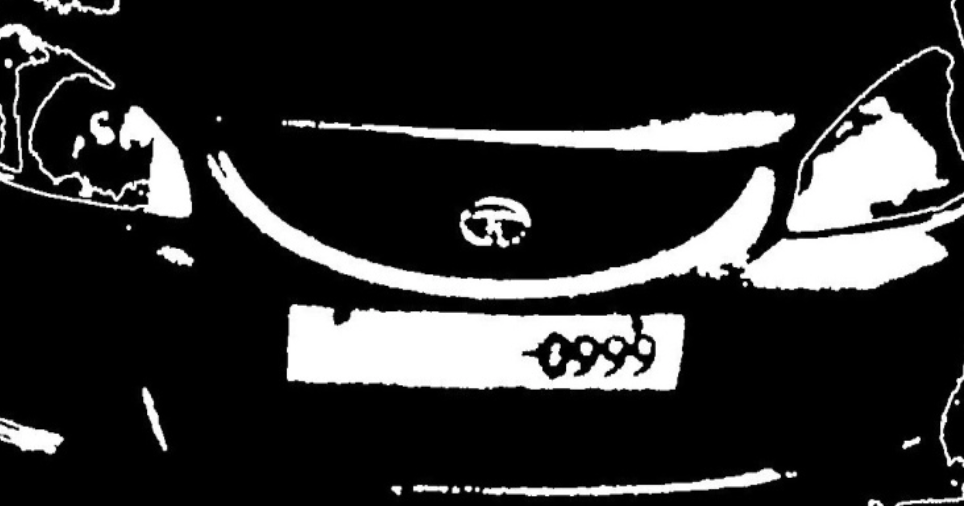
\includegraphics[width=88mm]{ext10.png}
	\caption{Imagem com as bordas encontradas e buracos preenchidos}
Fonte: Ahmed et al.~\cite{wafy2016efficient}
	\label{fig:wafy_example}
\end{figure}

O método proposto por Kaur~\cite{kaur2014efficient} foi testado com 120 diferentes imagens de veículos e obteve sucesso em 118 deles, mantendo um percentual de 98.33\%. O método implementado neste trabalho para a detecção da área da placa se baseia neste método.

Wafy e Madbouly~\cite{wafy2016efficient} propõe outra alternativa para a detecção da região da placa. Os autores se baseiam na distribuição semi-simétrica dos pontos de canto nas imagens de carros e placas e nas características morfológicas da região da placa.

O algoritmo de detectar as regiões candidatas consiste em quatro módulos. O primeiro módulo prepara a imagem para detecção aplicando pirâmides gaussianas para suavizar e remover ruídos da imagem. O segundo módulo detecta pontos de canto utilizando o detector de Harris. O terceiro módulo encontra uma linha vertical de simetria se baseando no fato de que uma imagem contendo uma placa de carro tem uma distribuição semi-simétrica de pontos de canto na placa. O quarto módulo procura verticalmente nas linhas simétricas para encontrar a região candidata que tem o maior número de pontos de canto. 

A solução proposta por Wafy e Madbouly~\cite{wafy2016efficient} teve uma taxa de acerto de 97,5\% no processo de detecção, com o maior tempo de execução para um dos processos sendo de
0,3s. Com estes resultados seria possível utilizar este método em aplicações de tempo real.

\section{Segmentação dos caracteres}

Em Abtahi et al.~\cite{abtahi2015deep} foram feitas novas abordagens para a
segmentação de caracteres em imagens. De acordo com eles, o método padrão de
segmentação baseado em projeção sofre com variações consideráveis na região da
placa ao redor dos caracteres, portanto estes autores propuseram duas abordagens.
A primeira é feita adaptando um método de aprendizado por reforço, criando um agente que
consiga achar os melhores caminhos para a segmentação.  A segunda abordagem usa
um método híbrido que utiliza a simplicidade e velocidade do método de projeção,
mas com o poder do aprendizado por reforço.

\section{Reconhecimento em sistema embarcado}

Com relação ao uso de sistema embarcado para executar o reconhecimento, Arth et
al.~\cite{arth2007real} trabalharam no desenvolvimento de um sistema de reconhecimento
de placas de carro em um processador de sinal digital (\emph{Digital Signal Processor}, DSP).
\emph{DSPs} são microprocessadores especializados em
processar sinais digitais como áudio ou vídeo em tempo real~\cite{yovits1993advances}. O processador utilizado
neste trabalho específico foi um \emph{Texas Instruments C64} com \emph{1MB} de \emph{cache RAM} e um outro bloco
de memória mais lento, \emph{SDRAM} de \emph{16MB}. O processador não possui câmera integrada mas permite a conexão de
uma fonte de vídeo analógica ou digital. Na solução implementada foi utilizada uma câmera com resolução de \emph{352x288 pixels}.

Com sua implementação, Arth et al.~\cite{arth2007real} foram capazes de conseguir localizar a placa em
\emph{7,30 ms}, levando mais aproximadamente \emph{1 ms} para identificar cada caractere. Não é informado, no artigo,
a taxa de sucesso de cada reconhecimento. Os autores ainda
concluem que pelo tempo de detecção da placa ser superior ao tempo de
reconhecimento dos caracteres, este algoritmo deve ser melhorado.

\section{Análise dos trabalhos}

Analisando os trabalhos feitos na área, nota-se que por mais que os algoritmos variem,
a base da detecção de placas permanece parecida. Eles costumam ser divididos em pelo
menos duas partes, a localização da placa e a detecção dos caracteres. Inclusive, Ahmad et al~\cite{ahmad2015automatic}
misturou diferentes algoritmos, utilizando a localização de um e a detecção de
outro, demonstrando que os dois passos são bem independentes.

Pode-se notar que o reconhecimento de placas de carros é uma área bastante estudada,
com diversas abordagens diferentes e grande variação de resultados. Entretanto, um problema que ainda existe é a grande variação nas placas de diferentes países, no estilo, fonte, caracteres utilizados e padrão do texto. A solução deste problema é a criação de um método local de reconhecimento de placas.
